\documentclass{llncs}

% name of the language
\newcommand{\lang}[0]{MediatE}

\title{A New Coordination Language \lang{}}

\author{Yi Li\and Meng Sun}
\institute{LMAM and Department of Informatics, School of Mathematical Sciences, Peking University, Beijing, China \\
\email{liyi\_math@pku.edu.cn, sunmeng@math.pku.edu.cn}
}


\usepackage{listings}
\usepackage{textcomp}
\usepackage{xcolor}
\usepackage{enumitem}
\usepackage{amssymb}
\usepackage{empheq}
\usepackage{mathpartir}
% \usepackage{pxfonts}
\usepackage{fancybox}
\usepackage{algorithmic}
\usepackage{algorithm}
\usepackage[normalem]{ulem}
\usepackage{tikz}

\makeatletter
\newenvironment{CenteredBox}{% 
\begin{Sbox}}{% Save the content in a box
\end{Sbox}\centerline{\parbox{\wd\@Sbox}{\TheSbox}}}% And output it centered
\makeatother

\renewcommand{\ttdefault}{pxtt}

\newtheorem{formalization}{Formalization}

\lstdefinelanguage{newlang}{
    keywords = {
        automaton,
        system,
        type,
        in, out,
        variables, transitions, statements, components, connections, 
        internals,
        begin, end,
        return,
        init,
        perform, as,
        int, bool, char, enum, real
    },
    alsodigit = {-}
}

\lstset{
    basicstyle=\small\ttfamily, 
    numbers=left,
    numberstyle=\scriptsize,
    columns=flexible,
    numbersep=10pt,
    tabsize=2,
    extendedchars=true,         %
    breaklines=true,
    keywordstyle=\bfseries,
    stringstyle=\color{white}\ttfamily, % Farbe der String
    xleftmargin=17pt,
    framexleftmargin=17pt,
    framexrightmargin=5pt,
    framexbottommargin=4pt,
    % backgroundcolor=\color{lightgray},
    showstringspaces=false,
    language=newlang
}

% terminal symbols
\newcommand{\tsym}[1]{\:\mbox{\texttt{#1}}\:}
% non-terminal symbols
\newcommand{\ntsym}[1]{\:\langle\mbox{\emph{#1}}\rangle\:}


\newcommand*\widefbox[1]{\fbox{\hspace{1em}#1\hspace{1em}}}

\newenvironment{bnf}{%
    % \vspace{-1em}
    \setkeys{EmphEqEnv}{align*}%
    \setkeys{EmphEqOpt}{box=\widefbox}%
    \EmphEqMainEnv%
}{
    \endEmphEqMainEnv
    % \vspace{-1em}
}

\newcommand{\subtype}[0]{\preccurlyeq}

\newcommand\T{\rule{0pt}{2.6ex}}       % Top strut
\newcommand\B{\rule[-1.2ex]{0pt}{0pt}} % Bottom strut

\newcommand\smalltitle[1]{
    \vspace{0.2cm}
    \noindent\emph{{#1}.}
}

\begin{document}

\maketitle

\begin{abstract}
In this paper, we presents \lang{} that intends to provide a two-step modeling approach in component-based software engineering. \lang{} is a formal modeling language where we take \emph{automata}  as basic behavioral units. Equipped with a rich-featured type system and template mechanism, automata are capable to model generic components and connectors. Such components and connectors are organized through \emph{systems}. The language makes it easy to construct complex models with simply reuse of existing elements, where their formal nature are still maintained. 
\end{abstract}

\section{Introduction}

% \section{Overview}

% \begin{figure}
%     \begin{bnf}
%         \ntsym{program} &::=& (\ntsym{typeDef}|\ntsym{funcDef}|\ntsym{automataDef}|\ntsym{systemDef})^* \\
%         \ntsym{typeDef} &::=& \tsym{typedef} \ntsym{type} \tsym{as} \ntsym{name} \\
%         \ntsym{funcDef} &::=& \tsym{function} \ntsym{template} \ntsym{name} \ntsym{interface} \ntsym{funcBody} \\
%     \end{bnf}
%     \caption{Abstract Syntax Tree}
% \end{figure}

The goal of this language \lang{} mainly focus on:

\begin{enumerate}
    \item Compositional Verification.
\end{enumerate}
\section{The Grammar}
\label{lbl:grammar}

In this section, we mainly focus on the syntax of our language, it is divided into different parts and basically described in  \emph{Extended Backus-Naur form (EBNF)}.

Let's introduce the overview of this language first.

\begin{bnf}
    \ntsym{program} &::= & [\ntsym{statement}]^* \\
    \ntsym{statement} &::=& \ntsym{importStmt} | \ntsym{typedefStmt} | \ntsym{functionStmt} \\
    &|& \ntsym{channelStmt} | \ntsym{componentStmt} \\
    &|& \ntsym{connectorStmt} \\
\end{bnf}

\subsection{Type System}

The basic idea behind this type system is that we try to satisfy both researchers and programmers.

\begin{bnf}
    \ntsym{primitiveType} &::= & \tsym{int}[\ntsym{term}\tsym{..}\ntsym{term}] \\
    & | & \tsym{double} | \tsym{char} | \tsym{bool} | \tsym{NULL} \\
    & | & \tsym{enum} {\{} \ntsym{identifier}^+\tsym{\}} \\ 
    & | & \ntsym{identifier} \\
    \ntsym{extendedType} &::= & \ntsym{primitiveType} \\
    & | & \ntsym{type} \tsym{$|$} \ntsym{type} \\
    & | & \tsym{array} \ntsym{extendedType} \tsym{[} \ntsym{term} \tsym{]}\\
    & | & \tsym{map} \tsym{[} \ntsym{extendedType}\tsym{]} \ntsym{type}\\
    & | & \tsym{struct} \tsym{\{} (\ntsym{identifier} \tsym{:} \ntsym{type})^+ \tsym{\}}\\
\end{bnf}

% TODO is raw type a common name ? needs some googling

\begin{definition}[Finite Types]
    A type in \lang{} is \emph{finite} iff. it has a finite value domain.
\end{definition}


\noindent\emph{Primitive Type.} \lang{} provides built-in support for common primitive types, they are,
\begin{itemize}
    \item \emph{Int}. Similar to  
    \item \emph{Double.}
    \item \emph{Bool.} Boolean variables.
    \item \emph{Enum.} An \emph{enumeration} is a finite collection of unique identifiers.
    \item \emph{NULL.} For simplicity, in \lang{} we don't have pointers references, however, sometimes an empty value is strongly required to denote uninitialized value. Consequently, we define a single-value type NULL, of which the only possible value is \emph{null}.
\end{itemize}

\noindent\emph{Extended Type.} Extended type offers an approach to contruct complex data types with simpler ones. Four extending patterns are introduced as follows,
\begin{itemize}
    \item \emph{Union}. The \emph{union} operator `$|$' is designed to combine two \emph{disjoint} types as a more complicated one. This is similar to the union type in C language but much easier to use.
    \item \emph{Array} and \emph{Slice}. An \emph{array} $T$[n] is a finite ordered collection containing exactly $n$ elements of type $T$. Moreover, a \emph{slice} is an array of which the capacity is not specified.
    \item \emph{Map}. A \emph{map }[$T_{key}$] $T_{val}$ is a dictionary that maps a key of type $T_{key}$ to a value of type $T_{val}$.
    \item \emph{Struct}. A \emph{struct }\{$field_1:T_1,\cdots,field_n:T_n$\} contain $n$ fields, each has a particular type $T_i$ and a unique identifier $id_i$.
\end{itemize}

Type systems often differ greatly between formal models and real-world programming languages. For example, PRISM\cite{KwiatkowskaCav2011}, ..

% TODO: in popular standards, a system may contains different safety/security level. 

In \lang's type system, most of basic types are finite except for the unlimited integers and doubles. Besides, extended types are also finite if they are based on finite ones.

% typing rules

\begin{definition}[Subtyping]
    Type $T_1$ is a subtype of $T_2$, denoted by $T_1\subtype
 T_2$, iff. a value of type $T_1$ can be converted to a value of type $T_2$ losslessly.
\end{definition}

\begin{mathpar}
    \inferrule* [right=S-FiniteInt] {l_1,u_1,l_2,u_2 \in \mathbb{Z}, l_1\leq u_1\land l_2\geq u_2}{\mbox{int $l_1$ .. $u_1$} \subtype \mbox{int $l_2$ .. $u_2$}} \\
    \inferrule* [right=S-Enum] {n \in \mathbb{Z}}{\mbox{enun \{ $item_0,\cdots,item_{n-1}$\}} \subtype \mbox{int 0 .. (n - 1)}} \\
    \inferrule* [right=S-Bool] {.}{\mbox{bool} \subtype \mbox{int 0 .. 1}} \\
    \inferrule* [right=S-Int] {l,u \in \mathbb{Z}}{\mbox{int $l$ .. $u$} \subtype \mbox{int}}\\
    \inferrule* [right=S-Union] {T_1\subtype T_3, T_2\subtype T_4}{T_1 | T_2 \subtype T_3 | T_4 } \\
\end{mathpar}

\begin{definition}[Abstract and Concrete Types]
    The types which have default values specified are called concrete types. And on contrary, those without default values are termed abstract types.
\end{definition}
\begin{bnf}
    \ntsym{concreteType} & ::= & \ntsym{extendedType} \tsym{init} \ntsym{term}
\end{bnf}

In most programming languages, a non-reference type has a built-in default value. However, such values are not specified by programmers, and sometimes may lead to unexpected behavior.

\subsection{Terms}

\begin{bnf}
    \ntsym{term} &::=& \ntsym{termPrimitive} \\
    &|& \ntsym{term} \tsym{+} \ntsym{term} | \ntsym{term} \tsym{-} \ntsym{term} \\
    &|& \ntsym{term} \tsym{*} \ntsym{term} | \ntsym{term} \tsym{/} \ntsym{term} \\
    &|& \tsym{!} \ntsym{term} \\
    &|& \ntsym{identifier} \tsym{(} \ntsym{term}^* \tsym{)} \\
    &|& \ntsym{term} \tsym{[} \ntsym{term} \tsym{]} \\
    &|& \ntsym{term} \tsym{.} \ntsym{identifier} \\
\end{bnf}

\begin{mathpar}
    \inferrule* [right=T-Call]{t_1:T_1,\cdots,t_n,T_n,f:T_1\rightarrow \cdots T_n\rightarrow T}{f(t_1,\cdots,t_n):T} \\
    \inferrule* [right=T-Array]{t_{arr}:T\:[n],0\leq i<n}{t_{arr}[i]:T} \\
    \inferrule* [right=T-Slice]{t_{slice}:T\:[\:],0\leq i< len(t_{slice})}{t_{slice}[i]:T} \\
    \inferrule* [right=T-Map]{t_{map}:\mbox{map }[T_1]\:T_2,t_{key}:T_1}{t_{map}[t_{key}]:T_2}\\
    \inferrule* [right=T-struct]{t_{struct}:\mbox{struct }\{field_1:T_1,\cdots,field_n:T_n\},1\leq i\leq n}{t_{struct}.field_{i}:T_i}
\end{mathpar}

Rules of operators (e.g. $+,-,*$) are not presented here. That's mainly due their abstract nature. In \lang{}, native semantics of numeric operators are absent on syntax level. In other words, we have to manually override these operators as functions, for example.

\begin{example}[Operator Overriding]
    \begin{lstlisting}
native function operatorAdd (a:int,b:int):int;
native function <l1:int,l2:int,u1:int,u2:int> operatorAdd(a:int l1 .. u1, b:int l2 .. u2) : int (l1 + l2) .. (u1 + u2);
    \end{lstlisting}
\end{example}

% TODO: note that in the rules there some logic formulas. in practice, these formulas needs to be derived from guard conditions or else

\subsection{Channels and Components}

Channels are the atomic functional units in our language. A channel compries several parameters; a set of ports, either \emph{input} or \emph{output}; some private variables; and a series of \emph{ordered} transitions.

Essentially, behavior of a channel is encoded as a set of \emph{guarded transitions}. 

Before introducing the formal grammar of channels, we present a simple example here.

% \begin{example}[Asynchronous Buffer Channel].

% \end{example}

% \begin{lstlisting}
% channel <type T, int n> FIFO1 (in A T, out B T)
%     variables
%         buf (T | EMPTY) init EMPTY;
%     end variables

%     transitions
%         buf != EMPTY ->
%             A.reqRead, B.reqWrite := false, true;
%         buf == EMPTY ->
%             A.reqRead, B.reqWrite := true, false;

%         A.reqWrite && buf == EMPTY ->
%         begin
%             perform A;
%             buf := A;
%         end

%         B.reqRead && buf != EMPTY ->
%         begin
%             B := buf;
%             buf := EMPTY;
%             perform B;
%         end
%     end transitions
% end channel
% \end{lstlisting}

\begin{bnf}
    \ntsym{channel} & ::= & \tsym{channel}[\ntsym{template}]\ntsym{identifier} \stsym{(} \ntsym{port}^* \stsym{)}\\
    & & \tsym{\{} \ntsym{variables} \ntsym{transitions} \tsym{\}} \\
    \ntsym{port} & ::= & \ntsym{identifier} \tsym{:} (\tsym{in}|\tsym{out}) \ntsym{type} \\
\end{bnf}

Templates make it able to create a family of similar channels with a single definition. That is, we are able to declare a set of parameters in the channel's definition. And when creating channel instances, you have to specify concrete values to these parameters. A parameter here can be either a type identifier (decorated with prefix \textbf{type}), or a normal variable. 

\begin{bnf}
    \ntsym{template} & ::= & \tsym{$\langle$} \ntsym{param}^+ \tsym{$\rangle$} \\
    \ntsym{param} & ::= & (\tsym{type} | \ntsym{type}) \ntsym{identifier}
\end{bnf}

\noindent \emph{Variables.} Local variables can be declared in the \emph{variables} segement, and referenced in the \emph{trnasitions} segement. 

\begin{bnf}
    \ntsym{variables} & ::= & \tsym{variables} \tsym{\{} (\ntsym{identifier} \ntsym{type} [\tsym{init} \ntsym{term}])^* \tsym{\}}
\end{bnf}

\noindent \emph{Transitions.} A transition is a guarded command that is executed when 
\begin{bnf}
    \ntsym{transitions} & ::= & \tsym{transitions} \\
    & & (\ntsym{transition}|\ntsym{group})^* \\
    & & \tsym{end transitions} \\
    \ntsym{transition} & ::= & \ntsym{term} \rightarrow \\
    & & (\ntsym{statement} | \tsym{begin} \ntsym{statement}^+ \tsym{end})\\
    \ntsym{statement} & ::= & \ntsym{identifier}^+\tsym{:=}\ntsym{term}^+\\
    & | & \tsym{perform} \ntsym{identifier}^+ \\
    \ntsym{group} & ::= & \tsym{group} \ntsym{transition}^+ \tsym{end group}
\end{bnf}

\subsection{Connectors}

\begin{bnf}
    \ntsym{connector} & ::= & \tsym{connector}[\ntsym{params}]\ntsym{identifier} \stsym{(} \ntsym{ports} \stsym{)} \\
    & & [\ntsym{internal}] (\ntsym{connection})^+ \tsym{end connector} \\
    \ntsym{interal} & ::= & \tsym{internal} (\ntsym{identifier})^+ \\
    \ntsym{connection} & ::= & \ntsym{identifier} \tsym{(} \ntsym{identifier}^+ \tsym{)}
\end{bnf}
\section{Semantics}
\label{sec:semantics}

In the section, we introduce the formal semantics of \lang{} through the following steps. First we introduce the concept \emph{configuration} to describe the state of an automaton. Then we consider the formalizations proposed in Section. \ref{sec:syntax} and canonicalize them. Finally, based on the canonical form of automata, we show how define their semantics as \emph{transition systems}.

As we have mentioned before, systems are only composition of automata. Consequently, we will not introduce its formal semantics directly. But instead, we show how automata in a system are composed and flattened into a single automaton.

% TODO: a figure is required here

\subsection{Configurations of Automata}
\label{subsec:config}
In a \lang{} automaton, due to absence of locations, the state only depends on the values of its \emph{local variables} and \emph{adjoint variables}. First we introduce the definition of \emph{valuation} on a set of variables. Basically, a valuation is a function that maps variables to one of its valid values. To make things more clear, in the rest of the paper we use $\mathbb{D}$ to denote the set of all values of all types.

\begin{definition}[Valuation]
A valuation of a set of variables $V$ is defined as a function $v:V\rightarrow \mathbb{D}$ that satisfies $\forall x\in V,v(x)\in Dom(type(x))$. We denote the set of all possible valuations of $Vars$ by $Val(Vars)$.
\end{definition}

\begin{definition}[Configuration] A configuration of an automaton $A=\langle Ports,$ $Vars,Trans_G\rangle$ is defined as a tuple $(v_{loc},v_{adj})$ where $v_{loc}\in Val(Vars)$ is a valuation on local variables, and $v_{adj}\in Val(Adj(P))$ is a valuation on adjoint variables. We use $Conf(A)$ to denote all the configurations of $A$.
\end{definition}

With \emph{configuration}s formally given, it's easy to give mathematical descriptions on all the language elements in an automaton. We don't care about systems since they are not semantics units. Table. \ref{table:mathdesc} shows their mathematical descriptions where we assume that all the elements belong to an automaton $A$.

\begin{table}
    \caption{Mathematical Description of the Formalizations}
    \label{table:mathdesc}
    \centering
    \begin{tabular}{lcr}
        \hline
        Name & Formalization & Mathematical Description \T\B \\
        \hline
        \T Assignment Statement\hspace{0.5cm} & $s$ & $s:Conf(A)\rightarrow Conf(A)$  \\
        Transition & $g=g\rightarrow S$ & $g:Conf(A)\rightarrow Bool,S\in Statement^* $  \\
        Transition Group & $t_G=\{t_1,\cdots,t_n\}$ & $t_G\in P(TR)$ \\
        \B Enumeration & \texttt{enum {item$_1$, ..., item$_n$}} \\
        \hline
    \end{tabular}
\end{table}


\subsection{Canonical Form of Transitions and Automata}
\label{subsec:canonical}

It is clear that we can use various combination of transitions to, actually, describe the same thing. For example, \texttt{a := b; c := d} and \texttt{a, c := b, d}. These irregular transitions make lead to a non-intuitive algorithm we joining multiple automata. In this subsection we show how to canonicalize them.

\begin{definition}[Canonical Transitions]
A transition $t=g\rightarrow\{s_1,\cdots,s_n\}$ is canonical iff. its statements $\{s_i\}$ is an interleaving sequence of assignments and synchronizing statements which start from and end by assignments, e.g. \texttt{a := exp$_1$; sync A; b := exp$_2$; $\cdots$ \texttt{c := exp$_3$}}.
\end{definition}

Suppose $g\rightarrow\{s_1,\cdots,s_n\}$ is a transition of automaton $A$, the following steps show how it is canonicalized,
\begin{description}
    \item[S1] If we can find a continuous subsequence $s_i,\cdots,s_j$ (where $s_k$ is an assignment statement for all $k= i,i+1,\cdots,j$, and $j>i$), we will merge them as a single one. Since an assignment statement is formalized as a function $f:Conf(A)\rightarrow Conf(A)$. Thus a list of multiple assignments $s_i,\cdots, s_j$ can be replaced using $s'=s_i\circ\cdots \circ s_j$.
    \item[S2] Keep going with \emph{S1} until there is no further subsequence to merge.
    \item[S3] Put identical assignments $id_{Conf(A)}$ into any adjacent synchronizing statements. Similarly, if the statements' list start from or end with a synchronizing statement, we should also use $id_{Conf(A)}$ to decorate its head and tail.
\end{description}

It's clear that once we found such a continuous subsequence, the merging operation will reduce the number of statements. Obviously, number of statements is initialized finite, so the looping algorithm always terminates within certain time.

\begin{definition}[Canonical Automata]
    An automaton $A=\langle Ports,$ $Vars,Trans_G\rangle$ is canonical iff. a) $Trans_G$ includes only one transition group and b) all transitions in this group are also canonical.
\end{definition}

Now we show how $Trans_G$ is reformed to make the automaton canonical.
Suppose $Trans_G$ is composed of a set of transition groups:
\begin{small}
\[
    \{t_{G_1}=\{g_{11}\rightarrow S_{11},\cdots, g_{1l_1}\rightarrow S_{1l_1}\},\cdots,t_{G_n}=\{g_{n1}\rightarrow S_{n1},\cdots,g_{nl_n}\rightarrow S_{nl_n}\}\}
\]
\end{small}

Informally speaking, once a transition in $t_{G_1}$ is activated, all the other transitions in $t_{G_i}(i>1)$ should be strictly prohibited from being fired. We use $activated(t_G)$ to denote the condition where at least one transition in $t_G$ is enabled, formalized as
\[
    activated(t_G=\{g_1\rightarrow S_1,\cdots, g_n\rightarrow S_n\}) = g_1\lor\cdots\lor g_n
\]
Then we can generate the new set of transitions with no dependency on priority as followings.
\begin{small}
\begin{eqnarray*}
    g_{11}\rightarrow S_{11},&\cdots&,g_{1l_1}\rightarrow S_{1l_1}, \\
    g_{21}\land \lnot activated(t_{G_1})\rightarrow S_{21}, &\cdots&, g_{2l_2} \land \lnot activated(t_{G_1})\rightarrow S_{2l_2}, \cdots \\
    g_{n1}\land \lnot activated(t_{G_1},\cdots,t_{G_{n-1}})\rightarrow S_{n1}, &\cdots&, g_{nl_n} \land \lnot activated(t_{G_1},\cdots,t_{G_{n-1}})\rightarrow S_{nl_n} \\
\end{eqnarray*}
\end{small}
To simplify the equations, we use $activated(t_{G_1},\cdots,t_{G_{n-1}})$ to indicate that at least one group in $t_{G_1},\cdots,t_{G_{n-1}}$ is activated. It's equivalent form is $activated(t_{G_1})\lor\cdots\lor activated(t_{G_{n-1}})$. 
\subsection{From System to Automaton}
\label{subsec:composition}

System in \lang{} provides an approach to construct hierarchical models with automata (declared as \emph{components} and \emph{connectors}). In this section, we present the algorithms to flat the hierarchical model as a typical automaton.

Algorithm \ref{alg:compose}. shows how a system is flattened as an automaton, where we assume that all the sub-automata are canonical. First we refactor all the variables in its sub-automata to avoid name conflicts, so that transitions will not suffer from ambiguity.  Links are established by replacing occurrence of one port (or internal node) with the other.

After preparation of sub-automata, we then put all the transitions together, both \emph{internal} ones and \emph{external} ones.

Internal transitions are easy to handle. Since an internal transition do not synchronize with other transitions, we directly put all the internal transitions in all sub-automata into the flattened automaton.

External transitions, on the other hand, have to synchronize with its corresponding external transitions in other sub-automata. For example, when an automaton want to read some thing from a input port $P_1$, there must be another one that is writing something to its output port $P_2$ where $P_1$ and $P_2$ are overlapped in the system.

\begin{algorithm}[H]
    \caption{Flatting a System to an Automaton}
    \label{alg:compose}
    \begin{algorithmic}[1]
        \REQUIRE A system $S=\langle Ports, Automata, Internals, Links\rangle$
        \ENSURE An automaton $A$
        \STATE $A \leftarrow $ an empty automaton
        \STATE $A.Ports\leftarrow S.Ports$
        \STATE rename \emph{local variables} in $Automata=\{A_1,\cdots,A_n\}$ to avoid duplicated names
        \FOR {$l=\langle p_1,p_2\rangle\in S.Links$}
            \IF {$p_1\in S.Ports$}
                \STATE replace all occurrance of $p_2$ with $p_1$
            \ELSE
                \STATE replace all occurrance of $p_1$ with $p_2$
            \ENDIF
        \ENDFOR
        \STATE $ext\_trans\leftarrow \{\}$
        \FOR{$i\leftarrow 1,2,\cdots,n$}
            \STATE $A.Vars\leftarrow A.Vars + A_i.Vars$
            \STATE $A.Trans_G \leftarrow A.Trans_G + Internal(A_i.Trans_G)$
            \STATE $ext\_trans \leftarrow ext\_trans + External(A_i.Trans_G)$
        \ENDFOR
        \FOR{$set\_trans\in P(ext\_trans)$}
            \STATE $new\_edge\leftarrow \mbox{\texttt{Schedule}}(S, set\_trans)$ 
            \IF{\emph{new\_edge $\neq$ null}}
                \STATE $A.Trans_G = A.Trans_G + \{new\_edge\}$
            \ENDIF
        \ENDFOR
    \end{algorithmic}
\end{algorithm}

In \lang{} \emph{systems}, only adjoint variables (\texttt{reqRead, reqWrite} and \texttt{value}) are shared between automata. During synchronization, the most important principle is to make sure assignments to shared variables are executed before they are dereferenced. Basically, this is a topological sorting problem. A detailed algorithm is described in Algorithm \ref{alg:synchronize}.

\begin{algorithm}[t]
    \caption{Scheduling in a Synchronous Set of External Transitions}
    \label{alg:synchronize}
    \begin{algorithmic}[1]
        \REQUIRE A System $S$, a set of external canonical transitions $t_1,t_2,\cdots,t_n$
        \ENSURE A synchronized transition $t$
        \IF{$\{t_i\}$ don't belong to different automata or $\exists t_i$ is internal}
            \STATE $t\leftarrow null$
            \RETURN
        \ENDIF
        \STATE \emph{t.g, t.S} $\leftarrow \bigwedge_i t_i.g,\:\{\}$
        \STATE 
        \STATE  \emph{G} $\leftarrow$ a Graph $\langle V,E\rangle$
                \COMMENT{create a dependency graph}
        \FOR{$i\leftarrow 1,\cdots,n$}
            \STATE add $\bot_i, \top_i$ to \emph{G.V}
            \STATE \emph{lasts} $\leftarrow\{\bot_i\}$
            \FOR {$j\leftarrow 1, 3, \cdots, len(t_i.S) - 1$}
                \STATE \emph{ports} $\leftarrow$ all the synchronized ports in $t_i.S_{j+1}$
                \FOR {$l\in lasts, p\in ports$}
                    \IF {$p\not\in G.V$}
                        \STATE add $p$ to $G.V$
                    \ENDIF
                    \STATE add edge $l \xrightarrow{t_i.S_j} p$ to \emph{G.E}
                \ENDFOR 
            \ENDFOR
            \FOR {$l\in lasts$}
                \STATE add edge $l \xrightarrow{t_i.S_{len(t_i.S)}} \top_i$ to \emph{G.E}
            \ENDFOR 
        \ENDFOR
        \STATE
        \IF{($G$ comprises a ring) \emph{or} ($\exists v\in G.v\backslash S.Ports$ is a port whose \emph{degree} $\neq 4$)}
            \STATE $t\leftarrow null$
        \ELSE
            \STATE $t.S\leftarrow\{$ select all the statements in $G.E$ using topological sort $\}$
            \STATE $\forall P\in G.v\backslash S.Ports$ replace \texttt{sync P} in $t.S$ with \\ \hspace{1em} \texttt{P.reqRead, P.reqWrite := false, false}
        \ENDIF
    \end{algorithmic}
\end{algorithm}

Algorithm. \ref{alg:synchronize} does not always produce a synchronized transitions. Line 25 shows several situations where the synchronization process fails:
\begin{enumerate}
    \item The dependency graph includes a \emph{ring}, which is a sign of \emph{circular dependencies}. For example, transition \texttt{g$_1$ -> \{sync A;sync B;\}} and transition \texttt{g$_2$ -> \{sync B;sync A;\}}, where both ports require to be triggered first.
    \item The dependency graph includes a non-trivial vertex (neither $\bot$ nor $\top$) whose degree is not equal to $4$. In other words, a port is not properly synchronized or synchronized with more than two transitions (as mentioned in Section. \ref{subsec:system}, any communication happens only between two automata).
\end{enumerate}

Topological sorting, as we all knows, may generate different schedules for the same dependency graph. The following theorem shows that all these schedules are equivalent as transition statements.

\begin{theorem}[Equivalence between Schedules] If two set of assignment statements $S_1, S_2$ are generated from the same set of external transitions, they have exactly the same behavior (i.e. $S_1$ and $S_2$ will lead to the same result when executed under the same configuration).
\end{theorem}

\subsection{Automaton as Labelled Transition System}

With all the language elements properly formalized, now we introduce the formal semantics of \emph{automata} based on \emph{labelled transition system}.

\begin{definition}[Labelled Transition System, LTS]
    A transition system is a tuple $(S,\Sigma,\rightarrow,s_0)$ where $S$ is a set of states with initial state $s_0\in S$, $\Sigma$ is a set of actions, and $\rightarrow\subseteq S\times\Sigma\times S$ is a set of transitions. For simplicity reasons, we use $s\xrightarrow{a} s'$ to denote $(s,a,s')\in\rightarrow$.
\end{definition}

Suppose $A=\langle Ports, Vars, Trans_G\rangle$ is an automaton, its semantics can be captured by a labelled transition system $\langle S_A, \Sigma_A,\rightarrow_A,s_0\rangle$ where
\begin{itemize}
    \item $S_A$ is the set of all configurations of $A$.
    \item $s_0$ is the initial configuration where all variables (except \texttt{reqRead} and \texttt{reqWrite}) are initialized with their default value, and \texttt{reqRead} and \texttt{reqWrite} are initialized as \texttt{false}.
    \item $\Sigma_A=\{i\}\cup P(Ports)$ is the set of all actions.
    \item $\rightarrow_A\subseteq S_A\times \Sigma_A\times S_A$ is a set of transitions constructed by the following rules.
\end{itemize}

\begin{mathpar}
    \inferrule* [right=R-InputStatus] {p\in P_{in}}{(v_{loc}, v_{adj})\xrightarrow{}_A(v_{loc},v_{adj}[p.reqWrite\mapsto \lnot p.reqWrite])} \\
    \inferrule* [right=R-InputValue] {p\in P_{in}, val\in Dom(Type(p.value))}{(v_{loc}, v_{adj})\xrightarrow{}_A(v_{loc},v_{adj}[p.value\mapsto val])} \\
    \inferrule* [right=R-OutputStatus] {p\in P_{out}}{(v_{loc}, v_{adj})\xrightarrow{}_A(v_{loc},v_{adj}[p.reqRead\mapsto \lnot p.reqRead])} \\
    \inferrule* [right=R-Internal] {\{g\rightarrow \{s\}\}\in Trans_G\mbox{ is internal}}{(v_{loc}, v_{adj})\xrightarrow{i}_A s(v_{loc},v_{adj})} \\
    \inferrule* [right=R-External] {\{g\rightarrow S\}\in Trans_G\mbox{ is external, } \{s_1,\cdots,s_n\}\mbox{ are the assignments in $S$} \\\vspace{0.2em} \{p_1,\cdots,p_m\}\mbox{ are the synchronized ports}}{(v_{loc}, v_{adj})\xrightarrow{\{p_1,\cdots,p_m\}}_A s_n\circ\cdots\circ s_1(v_{loc},v_{adj})} \\
\end{mathpar}

The first three rules describe the potential change of context, i.e. the adjoint variables. R-InputStatus and R-OutputStatus shows that the reading status of an output port and status of an input port may changed by the context randomly. And R-InputValue shows that the value of an input port may also be updated.

The rule R-Internal models the internal transitions in $Trans_G$. As illustrated previously, an internal transition doesn't contains any synchronizing statement. So its canonical form comprises only one assignment $s$. Firing such a transition will simply apply $s$ to the current configuration.

Meanwhile, R-External models the external transitions, where the automaton need to interact with its context. Fortunately, since all the context change are captured by the first three rules, we can simply regard the context as another set of local variables. Consequently, the only difference between an internal transition and an external transitions is that the later may contains multiple assignments.
\section{Case Study}
\label{sec:casestudy}

In modern distributed computing frameworks (e.g. MPI\cite{mpibook} and ZooKeeper\cite{JunqueiraZab2011}), \emph{leader election} plays an important role to organize multiple servers efficiently and consistently. This section shows how a classical leader election algorithm is modeled and reused to coordinate other components in \lang{}.

\cite{HagitDistributed2004} proposed a classical algorithm for a typical leader election scenario, as shown in Fig. \ref{fig:leaderelection}. Distributed processes are organized as an \emph{asynchronous unidirectional} ring where communication takes place only between adjacent processes and following certain direction (indicated by the arrows on edges in Fig. \ref{fig:leaderelection} (a)).

\begin{figure}
	\centering
	\resizebox{.8\textwidth}{!}{
        \tikzstyle{node}=[
    circle,
    draw
]

\begin{tikzpicture}[remember picture]
    \def \n {5}
    \def \radius {2cm}
    \def \margin {11} % margin in angles, depends on the radius

    \foreach \s in {1,...,\n}
    {
    \node[draw, circle] at ({360/\n * (\s - 1)}:\radius) {$P_\s$};
    \draw[<-, >=latex] ({360/\n * (\s - 1)+\margin}:\radius) 
        arc ({360/\n * (\s - 1)+\margin}:{360/\n * (\s)-\margin}:\radius);
    }

    \node[draw, rectangle, minimum width=4cm] at (6,0) {
        \begin{tabular}{c}
            \\
            Process ($P_i$) \\
             \\
            \begin{tikzpicture}[remember picture]
                \node [draw, rectangle, minimum width=3cm, minimum height=1cm] (connector) at (0,0) {\texttt{election\_module}};
            \end{tikzpicture} \\
            \\
            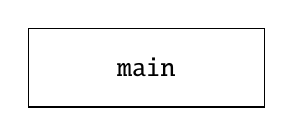
\begin{tikzpicture}[remember picture]
                \node [draw, rectangle, minimum width=3cm, minimum height=1cm] (component) at (0,0) {\texttt{main}};
            \end{tikzpicture}
            \vspace{0.5em}
        \end{tabular}
        };
    
    \draw[->, >=latex] (3,0.3) -- (connector) node[midway, above, xshift=-0.35cm] {\texttt{left}} ;
    \draw[->, >=latex] (connector) -- (9,0.3) node[midway, above, xshift=0.3cm] {\texttt{right}};
    \draw[<->, >=latex] (component) -- (connector) ;
\end{tikzpicture}
    }
	\caption{(a) Topology of an Asynchronous Ring and (b) Structure of a Process}
	\label{fig:leaderelection}
\end{figure}

The algorithm has the following steps:
\begin{enumerate}
	\item Each process sends a voting message including its own \emph{id} to its successor.
	\item A process, when receives a voting message, will
	\begin{itemize}
		\item forward the message to its successor if it contains a larger \emph{id} than itself,
		\item ignore the message if it contains a smaller \emph{id} than itself, and
		\item take itself as a leader if it contains the same \emph{id} with itself, and send an acknowledgement message to this successor, which will be spread over around the ring.
	\end{itemize} 
\end{enumerate}

Here we formalize this algorithm through a more general approach. Leader election is encapsulated as the \texttt{election\_module}. A computing module \texttt{worker},  attached to the \texttt{election\_module}, is an implementation of the working process. 

Two types of messages, \texttt{msgVote} and \texttt{msgLocal}, are supported when formalizing this architecture. Voting messages \texttt{msgVote} are transferred between the processes. A voting message carries two fields, \emph{vtype} that declares the stage of leader election (either it is still voting or some process has already been acknowledged) and \emph{id} is an identifier of the current leader (if it exists). On the other hand, \texttt{msgLocal} is used when a process communicates with its corresponding worker.
\begin{example}[The Election Module] The following automaton shows how the election algorithm is implemented in \lang{}. Due to the space limit, we omit some transitions here. A full version can be found at \cite{medmodels}.
\begin{lstlisting}[basicstyle=\scriptsize\ttfamily]
automaton <id:int> election_module ( left : in msgVote, right : out msgVote,
	query : out msgLocal
) {
	variables {
		leaderStatus : enum { pending, acknowledged } init pending;
		buffer : (voteMsg | NULL) init {vtype: vote, id:id};
		leaderId : (int | NULL) init null;
	}
	transitions {
		(buffer != null)&&(buffer.vtype == vote)&&(buffer.id < id) -> {buffer := null;}
		(buffer != null)&&(buffer.vtype == vote)&&(buffer.id == id) -> {buffer.vtype := ack;}
		(buffer != null)&&(buffer.vtype == ack)&&(buffer.id < id) -> {
			// restart voting if the acknowledged leader has a smaller id
			buffer := { vtype: vote, id: id };
		}
		(buffer != null)&&(buffer.vtype == ack)&&(buffer.id >= id) -> {
			leaderStatus := acknowledged;
			leaderId := buffer.id;
			buffer := buffer.id == id ? null : buffer;
		}
	}
}
\end{lstlisting}
\end{example}


The following code fragment encodes a parallel program containing 3 \emph{worker}s and 3 \emph{election\_module}s to organize the \emph{worker}s. It is a simplified version of the one in Fig. \ref{fig:leaderelection}. In this example, we do not focus on the implementation details on \emph{worker}s. Instead, we hope that any component with a proper interface could be embedded into this system. Consequently \emph{worker} is taken as a parameter of interface type.

\begin{lstlisting}[basicstyle=\scriptsize\ttfamily]
system <worker: interface (query:in msgLocal)> parallel_instance() {
	components {
		E1 : election_module<1>;
		E2 : election_module<2>;
		E3 : election_module<3>;
		C1, C2, C2 : worker;
	}	
	connections {
		Sync<msgVote>(E1.left, E2.right);
		Sync<msgVote>(E2.right, E3.left);
		Sync<msgVote>(E3.right,	E1.left);
		
		Sync<msgLocal>(C1,query,  E1.query);
		Sync<msgLocal>(C2,query,  E2.query);
		Sync<msgLocal>(C3,query,  E3.query);
	}
}
\end{lstlisting}

As we are modeling the leader election algorithm on a synchronous ring, only synchronous communication channels \emph{Sync}s are involved in this example. The implementation details of \texttt{Sync} can be found in  \cite{medmodels}.

\section{Conclusion and Future Work}

\bibliographystyle{splncs03}
\bibliography{fm}

\section*{Appendix}

\setcounter{theorem}{0}
\begin{theorem}[Equivalence between Schedules] If two set of assignment statements $S_1, S_2$ are generated from the same set of external transitions, they have exactly the same behavior (i.e. execution of $S_1$ and $S_2$ under the same configuration will lead to the same result.
\end{theorem}
\begin{proof}
    Apparently, when executing statements, all the changes on configurations come from \emph{assignments}. Once we successfully prove that for each assignment, its pre-configuration and post-configuration in $S_1$ and $S_2$ are exactly the same, we are able to finish this proof.
    
    In the following proof, we denote $S_1$ and $S_2$ by $S_1=\{s_1,\cdots,s_n\},S_2=\{s'_1,\cdots,s'_n\}$, and the automaton that a transition belongs to by $Automaton(s)$.
    \begin{enumerate}
        \item Let's come to the \emph{FIRST} assignment state $s$ in $S_1$ where shared variables is assigned. We assume that its corresponding statement in $S_2$ is $s'$. Comparing $s$ and $s'$, we have:
        \begin{enumerate}
            \item $s'$ is also the first assignment in $S_2$ which modifies \emph{this set} of variables.
            \emph{(A shared variable can be assigned in one of its owner, thus all assignments that modifies this variable belong to the same transition, and their order is strictly maintained.)}
            \item $s$ and $s'$ include no reference to other shared variables. \emph{(A shared variable can be dereferenced only when it has been assigned before, however $s$ is the first assignment which modifies a shared variable.)}
            \item In the pre-configuration of $s$ and $s'$, all the local variables of $Automaton(s)$ have the same evaluation. \emph{(Derived from the same reason in (a))}.
        \end{enumerate}
        Consequently, in the post-configuration of $s$ and $s'$, all the shared variables have the \emph{SAME} evaluation.

        \item Assume that all assignments (to shared variables) in $s_1,\cdots,s_i$ have been proved that satisfy the proposition, now we are going to prove that $s$, the first transition where shared variables are dereferenced in $s_{i+1},\cdots,s_n$ and its corresponding $s'$ also satisfy it.
    \end{enumerate}
\end{proof}

\end{document}